\documentclass[english, 11pt]{article}

\usepackage[T1]{fontenc}    % Riktig fontencoding
\usepackage[utf8]{inputenc} % Riktig tegnsett
\usepackage{babel}          % Ordelingsregler, osv
\usepackage{graphicx}       % Inkludere bilder
\usepackage{booktabs}       % Ordentlige tabeller
\usepackage{url}            % Skrive url-er
\usepackage{textcomp}       % Den greske bokstaven micro i text-mode
\usepackage{units}          % Skrive enheter riktig
\usepackage{float}          % Figurer dukker opp der du ber om
\usepackage{lipsum}         % Blindtekst
\usepackage{amsmath}        % Mattestæsj
\usepackage{listingsutf8}   % Kodetekst
\usepackage{verbatim}
\usepackage{subfigure}		% Flere fig. ved siden av hverandre
\usepackage[a4paper,margin=1.2in]{geometry}

\lstset{breaklines=True,numbers=left}

% JF i margen
\makeatletter
\renewcommand{\subsubsection}{\@startsection{subsubsection}{3}{-2cm}%
{-\baselineskip}{0.5\baselineskip}{\bf\large}}
\makeatother
\newcommand{\jf}[1]{\subsubsection*{JF #1}\vspace*{-2\baselineskip}}

% Skru av seksjonsnummerering
\setcounter{secnumdepth}{-1}

%, trim = 1cm 7cm 1cm 7cm % PDF-filer som bilde

\begin{document}

% Forside
\begin{titlepage}
\begin{center}

\textsc{\Large FYS4150 - Computational Physics}\\[0.5cm]
\rule{\linewidth}{0.5mm} \\[0.4cm]
{ \huge \bfseries  PROJECT 1}\\[0.10cm]
\rule{\linewidth}{0.5mm} \\[1.5cm]
\textsc{\Large Solving a differential equation using matrices}\\[1.5cm]
\textsc{}\\[1.5cm]

% Av hvem?

\begin{minipage}{0.49\textwidth}
    \begin{center} \large
        Jon Vegard Sparre\\ \url{jonvsp@uio.no} \\[0.8cm]
    \end{center}
\end{minipage}


\vfill

% Dato nederst
\large{Dato: \today}

\end{center}
\end{titlepage}

\abstract{In this project we're solving a differential equation with two different methods, with a algorithm for a tridiagonal matrix equation and with Armadillo's \verb|solve|-function. We look at the precision of the two methods and their speed.}
\\ \\
\emph{Note: I have collaborated with Henrik S. Limseth and Anne-Marthe Hovda in this project, but we have written our own programs and therefore deliver different reports.}

\section*{Exercise a)}

We're going to solve the one dimensional Poisson equation given on the form

\begin{equation}
    -u''(x) = f(x), \label{eq:diff}
\end{equation}

with Dirichlet boundary conditions. 

\paragraph{Rewriting of differential equation}
We'll show that we can write our differential equation (\ref{eq:diff}) as the matrix equation $ Av = \tilde b$. First we discretize our equation such that we have $-u_i'' = f_i$, then we use the three point formula for a second derivative to get

$$ -\frac{v_{i+1} + v_{i-1} - 2v_i}{h^2} = f_i, \quad \text{for } i=0,\ldots,n, $$

where we multiply both sides by $h^2$ such that we get $ \tilde b_i = h^2 f_i$ where $h = 1/(n+1) $. Then we simply write the matrix $A$ given in the exercise text and multiply it by $v$ to see what we get

\begin{align*}
	Av &=
	\left(\begin{matrix}
		2 & -1 & 0 & 0 &\ldots & 0 \\	
		-1 & 2 & -1 & 0 & \ldots & 0 \\
		0 & \ddots & \ddots & \ddots & \ddots & \vdots \\
		\vdots & \ddots & \ddots & \ddots & \ddots & 0 \\
		\vdots & \ddots & \ddots & \ddots & \ddots & -1 \\
		0 & \ldots & \ldots & 0 & -1 & 2 \\
	\end{matrix}\right)\left(
	\begin{matrix}
		v_1 \\ \vdots\\ \vdots \\ \vdots \\ v_n 
	\end{matrix} \right) \\
	&= \left(\begin{matrix}
		2v_1 & -v_2 & 0 & 0 &\ldots & 0 \\	
		-v_1 & 2v_2 & -v_3 & 0 & \ldots & 0 \\
		0 & \ddots & \ddots & \ddots & \ddots & \vdots \\
		\vdots & \ddots & \ddots & \ddots & \ddots & 0 \\
		\vdots & \ddots & \ddots & \ddots & \ddots & -v_n \\
		0 & \ldots & \ldots & 0 & -v_{n-1} & 2v_n \\
	\end{matrix}\right),
\end{align*}

where we recognize each row as the three point formula for the $i$-th component of $v$, \emph{e.g.} for $i=2$ we have

$$ -v_1 + 2v_2 -v_3 = \tilde b_2.$$

Thus we've shown that we can write the given differential equation as a system of linear equations.

\paragraph{Checking the given solution}
We're given the source term $f(x) = 100 e^{-10x}$, and we'll check if the solution $u(x) = 1-(1-e^{-10})x - e^{-10x}$ is correct, by inserting it into to Poisson's equation.

\begin{align*}
	u(x) &= 1-(1-e^{-10})x - e^{-10x} \\
	u'(x) &= (1-e^{-10}) + 10e^{-10x} \\
	u''(x) &= - 100e^{-10x} = -f(x).
\end{align*}
It is indeed correct and we can move on to next exercise!

\section*{Exercise b)}

The matrix $ A$ is rewritten as three column vectors in order to optimize our code, we can do this because the matrix $A$ is zero everywhere except at the three diagonals in the middle. We then get $n$ equations,
$$ a_i v_{i-1} + b_iv_i + c_i v_{i+1} = \tilde b_i.$$
To solve this we do a forward and then a backward substitution. The algorithm is described below

\begin{lstlisting}
Declaring variables
- Vectors a, b, c which is the subdiagonal, diagonal and superdiagonal of the matrix A.
- Vector v which is the one we're solving for.
- Vector f which is the source term in our diff. eq. discretized.

Setting initial conditions
...

We declare then a temporary varible which we'll use in the row reduction of A.
btemp = b_1;
The first element of v is then
v_1 = f_1/b_1

Make for loops that calculate v_i
for( i up to n):
    To do the substitution we need a temporary variable such that we can perform the row reduction of A, this we have to save this variable in order to do the backward substitution correct
    temp_i = c_{i-1} / btemp

    btemp = b_i - a_i*temp_i
    v_i = ( f_i - a_i * v_(i-1) ) / btemp

Then we do the backward substitution, starting from the second last element in v and moving backwards to i=1.
for(i=n-1 to  i>= 1):
    v_i = v_i - temp_(i+1) * v_(i+1)
\end{lstlisting}

For our calculation we have $8n$ FLOPS, $6n$ in the first for-loop and then $2n$ more in the second for-loop, a LU-decomposition requires $(2/3)n^3$ FLOPS so it's much more efficient to do it the way it's been done in this project.

I made a function to calculate the array $v$ which i named \verb|num_solve.cpp|, the main program is calling on this function when solving the problem using the tridiagonal solver. The main program is giving the parameters and variables $a$, $b$, $c$, $f$ and no. of grid points $n$, and also the object $v$ which is being filled by the function. All variables are called by reference, in order to avoid moving on large objects in the memory, except the integer number $n$.

\lstinputlisting[language=C++]{../num_solve.cpp}

The plots resulting from this method is shown in the end of this report together with the results from the method using Armadillo's \verb|solve|-function.

\section*{Exercise c)} In this part of the project we did an analysis of the relative error between our own numerical solution and the exact solution. We calculated the error as described in the exercise text,
$$ \epsilon_i \log_{10} \left( \left| \frac{v_i - u_i}{u_i} \right|  \right). $$
In my program it looked like this.\\

\lstinputlisting[language=C++, firstline=100, lastline=113]{../main.cpp}

Below we see table \ref{tab:error_max} with our maximum relative errors. We see that it decreases when $n$ is increasing, remember that the error is written as the logarithm of the relative error. In fig. \ref{fig:en101}, \ref{fig:en102}, \ref{fig:en103}, \ref{fig:en104} and \ref{fig:en105} we see the errors plotted as a function of $x$. When $n=10$ the error is constant equal $-1.1797$, which is what I should get for every $n$ if the algorithm is correct. This was discovered when Henrik and Anne-Marthe plotted the relative error between their solution from the LU-decomposition and the exact solution, since the LU-method is certainly correct the relative error between a numerical and exact solution should always, in this case, be a constant. As we can see from my own error this only happens for $n=10$, otherwise it increases with $x$. The bigger $n$ is the more the relative error increases, this may be due to some index-errors in my program which I haven't found.

\begin{table}[H]
  \centering
  \begin{tabular}{ c c }
    \toprule
    $n$ & $\epsilon_{\text max}$ \\
    \midrule
	$10$ &	$-1.1797$ \\
	$10^2$ & $-3.0880$ \\
	$10^3$ & $-5.0800$ \\
	$10^4$ & $-7.0753$ \\
	$10^5$ & $-8.3667$ \\
    \bottomrule
  \end{tabular}
  \caption{Maximum error for different $n$ when using LU-decomposition with forward and backward substitution. At $n=10^6$ our program crashes. Also note that the error is decreasing with increasing $n$.}
  \label{tab:error_max}
\end{table}

\begin{figure}[H]
    \centering
    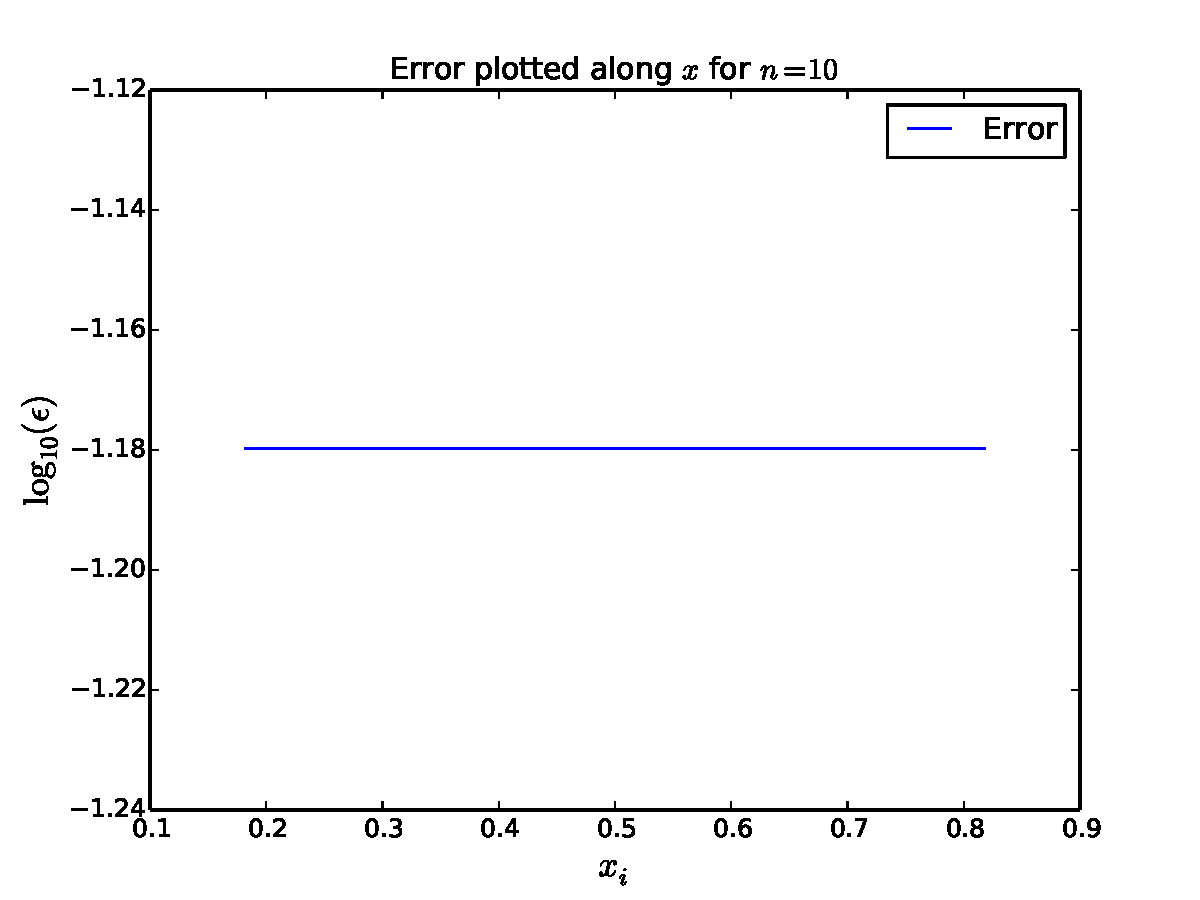
\includegraphics[width = .9\textwidth]{error_n_10.pdf}
    \caption{When $n=10$ the error is constant, this may be a coincidence. The error is quite big anyway, which we also see clearly in fig. \ref{fig:sol101}.}
    \label{fig:en101}
\end{figure}

\begin{figure}[H]
    \centering
    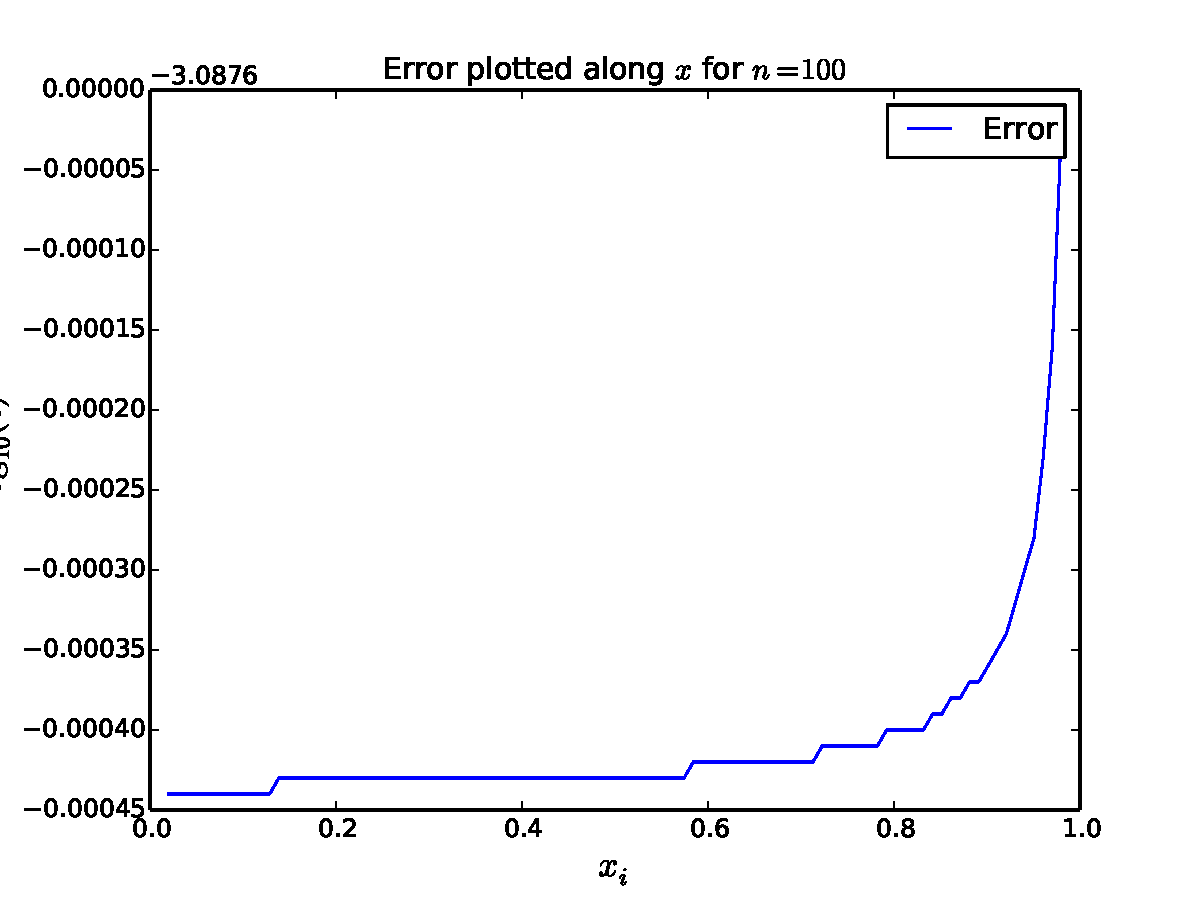
\includegraphics[width = .9\textwidth]{error_n_100.pdf}
    \caption{The relative error is for $n=100$ around $\log_{10}(-3.08)$, which is an expected improvement from $n=10$.}
    \label{fig:en102}
\end{figure}

\begin{figure}[H]
    \centering
    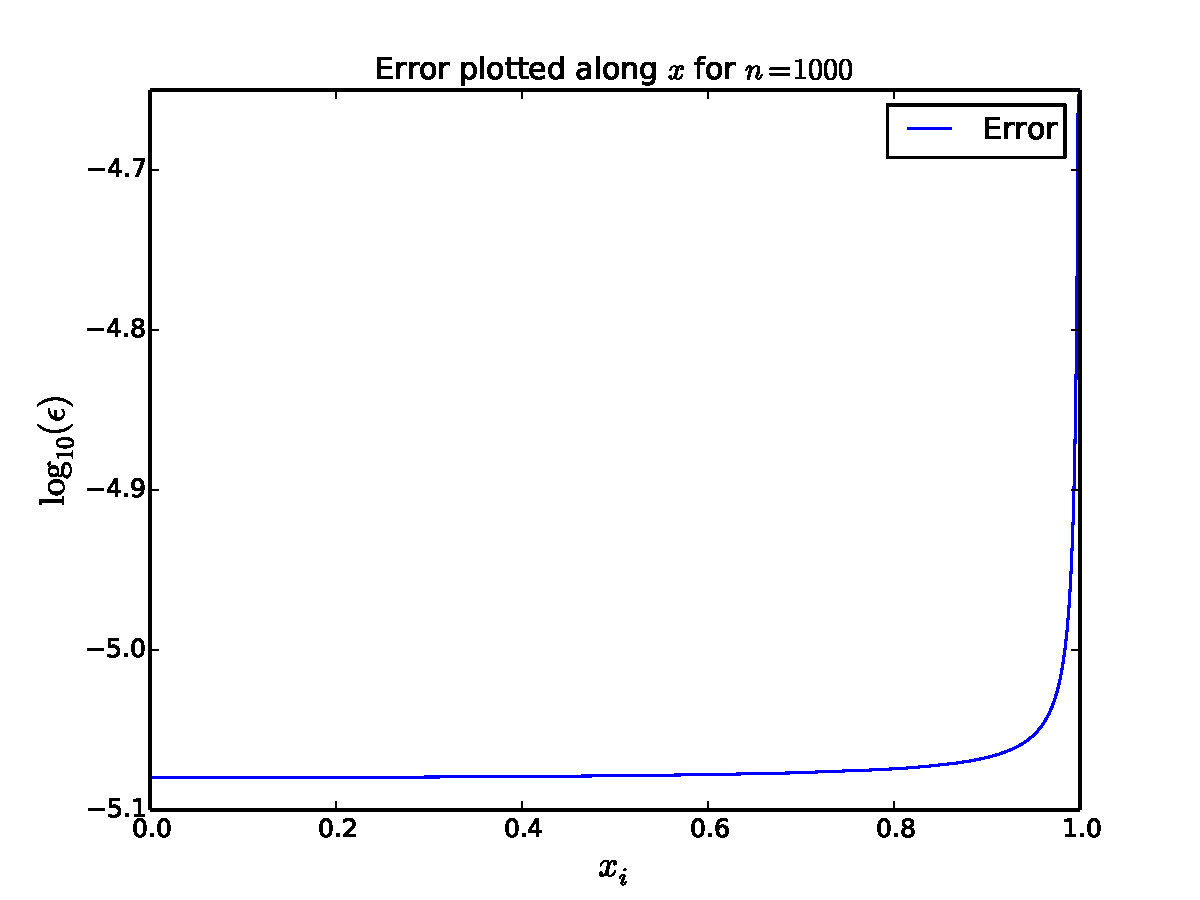
\includegraphics[width = .9\textwidth]{error_n_1000.pdf}
    \caption{Error plot for $n=10^3$}
    \label{fig:en103}
\end{figure}

\begin{figure}[H]
    \centering
    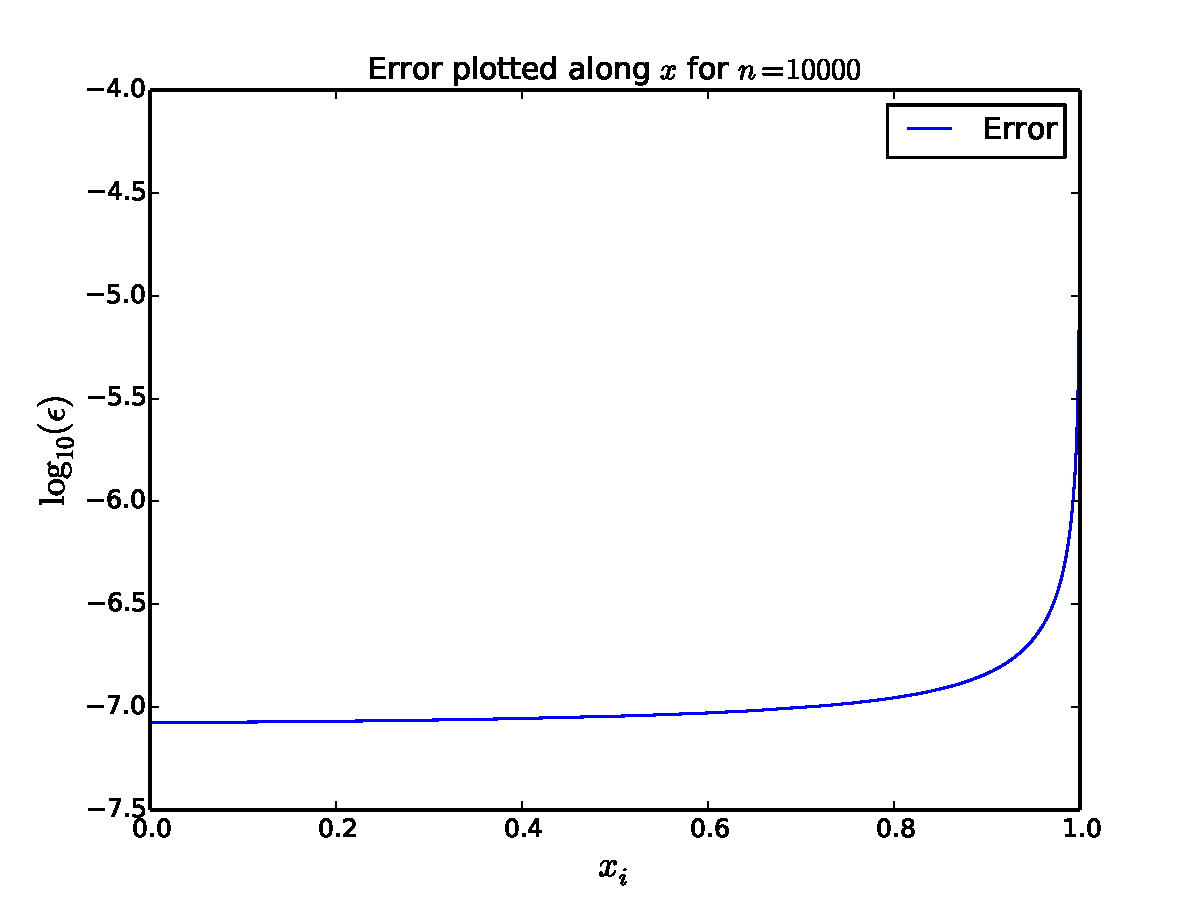
\includegraphics[width = .9\textwidth]{error_n_10000.pdf}
    \caption{Error plot for $n=10^4$}
    \label{fig:en104}
\end{figure}

\begin{figure}[H]
    \centering
    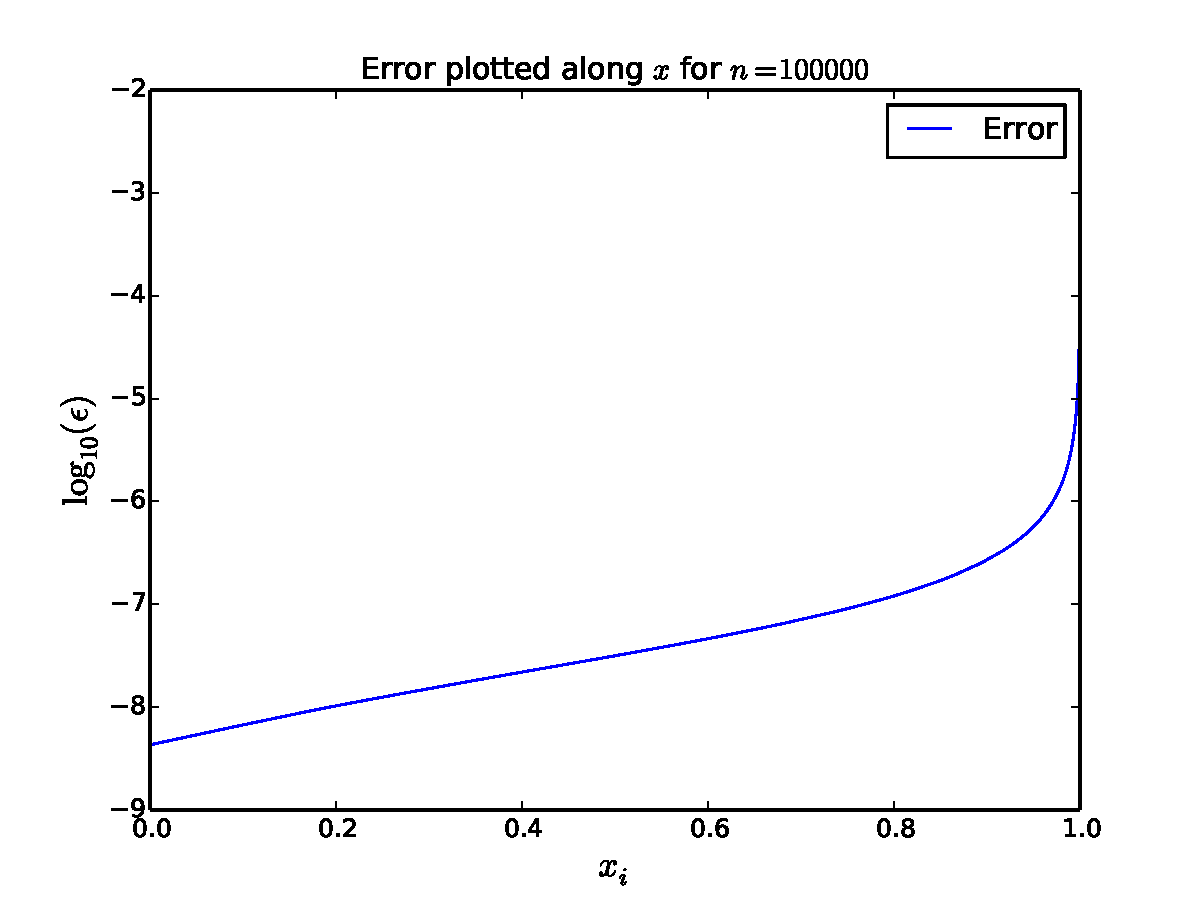
\includegraphics[width = .9\textwidth]{error_n_100000.pdf}
    \caption{Error plot for $n=10^5$. It seems like the numerical precision is decreasing when $n$ is getting too large.}
    \label{fig:en105}
\end{figure}

When we compare all our relative error-plots we see that the relative error is indeed decreasing for higher $n$, we also se that the relative error is always increasing a lot when $x\rightarrow 1$. This may be due to the accumulation of numerical error in the calculation.

\section*{Exercise d)} In this last part we're asked to compare our numerical results with the ones we get by using packages like Armadillo. First we can take a look at the function I made for solving the equation with Armadillo. The program is more or less self contained with comments that explain how it works. As we can see this program is much simpler than the one using, once we have initialized necessary objects we call on Armadillo's \verb|solve|-function and we're (almost) done, we have to shift the \verb|x2|-array in order to implement the boundary conditions correct.

\lstinputlisting[language=C++]{../arma_solve.cpp}

My main program calls on the different solving methods and saves the results as \verb|.txt|-files, see below. These files is read by a Python-script and plotted. The Python script is included at the end of the report and is self contained with comments.

\lstinputlisting[language=C++]{../main.cpp}

We'll now take a look at the results from our to methods. We have plotted three graphs in one plot: the exact solution, the solution from our tridiagonal solver and the solution from Armadillo's solver. We immediately see that Armadillo is useless when $n=10$. We get the same shape on the solution, but it is far too high, see fig. \ref{fig:sol101}. This happens again when $n=100$, but it's getting closer, see fig. \ref{fig:sol102}. We have to set $n=1000$ before we can say that Armadillo is giving any precision in it's calculations, with the tridiagonal solver the exact and numerical solution are so close that it's hard to distinguish between the two graphs.

The big difference in the precision of these two methods may be due to the number of floating point operations. The more FLOPS we have, the more numerical error we get in the final result because the error will accumulate.

\begin{figure}[H]
    \centering
    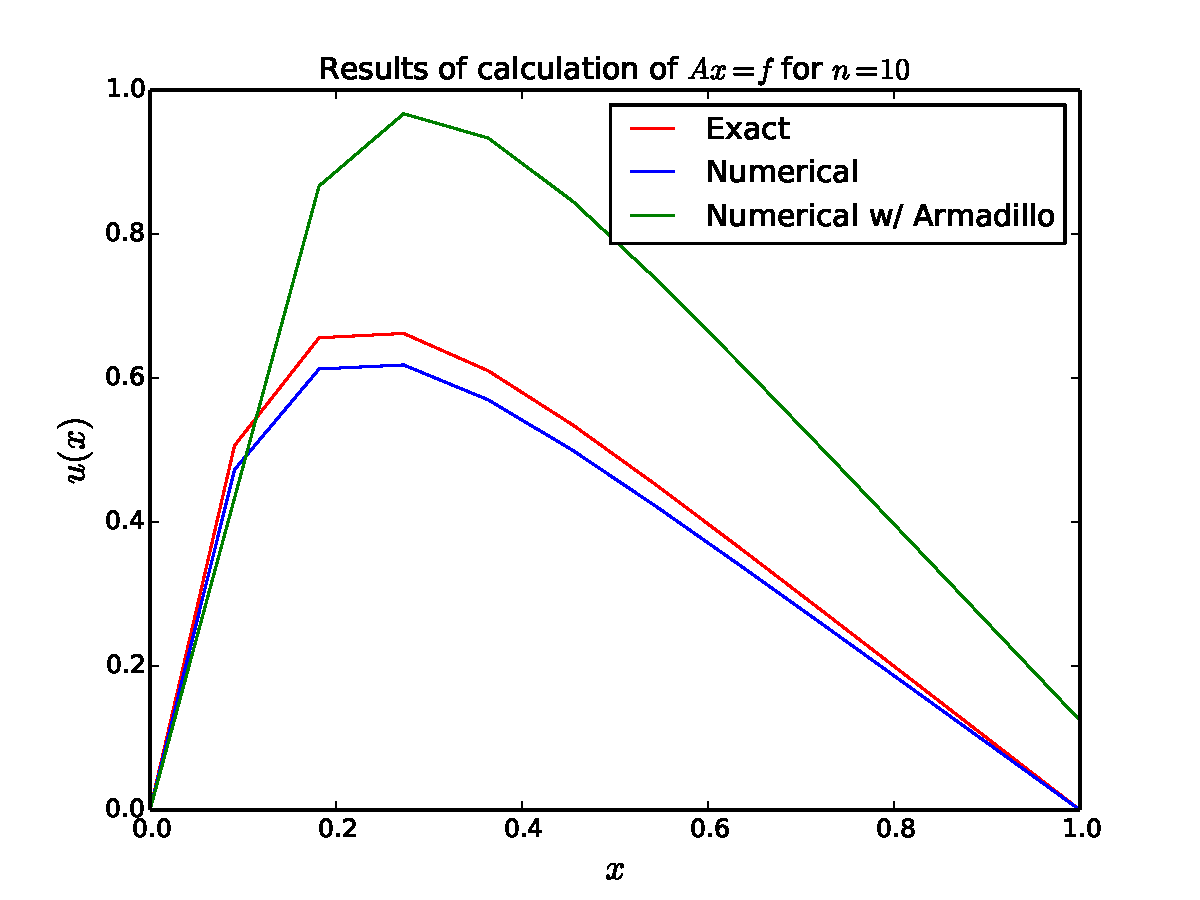
\includegraphics[width = .9\textwidth]{d_n_10.pdf}
    \caption{Numerical solution for $n=10$. Armadillo's function `solve' is pretty far off from the exact and the first numerical solution.}
    \label{fig:sol101}
\end{figure}

\begin{figure}[H]
    \centering
    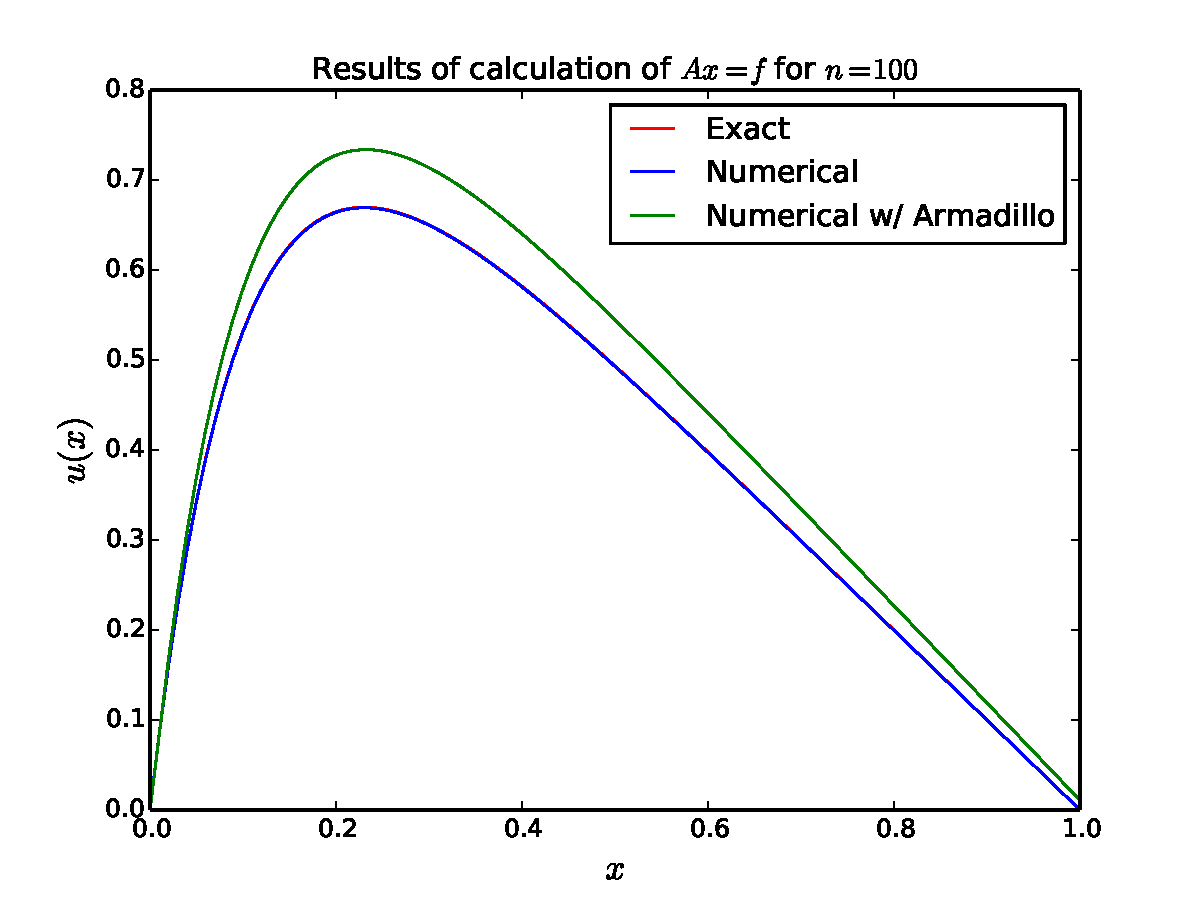
\includegraphics[width = .9\textwidth]{d_n_100.pdf}
    \caption{Numerical solution for $n=10^2$.}
    \label{fig:sol102}
\end{figure}

\begin{figure}[H]
    \centering
    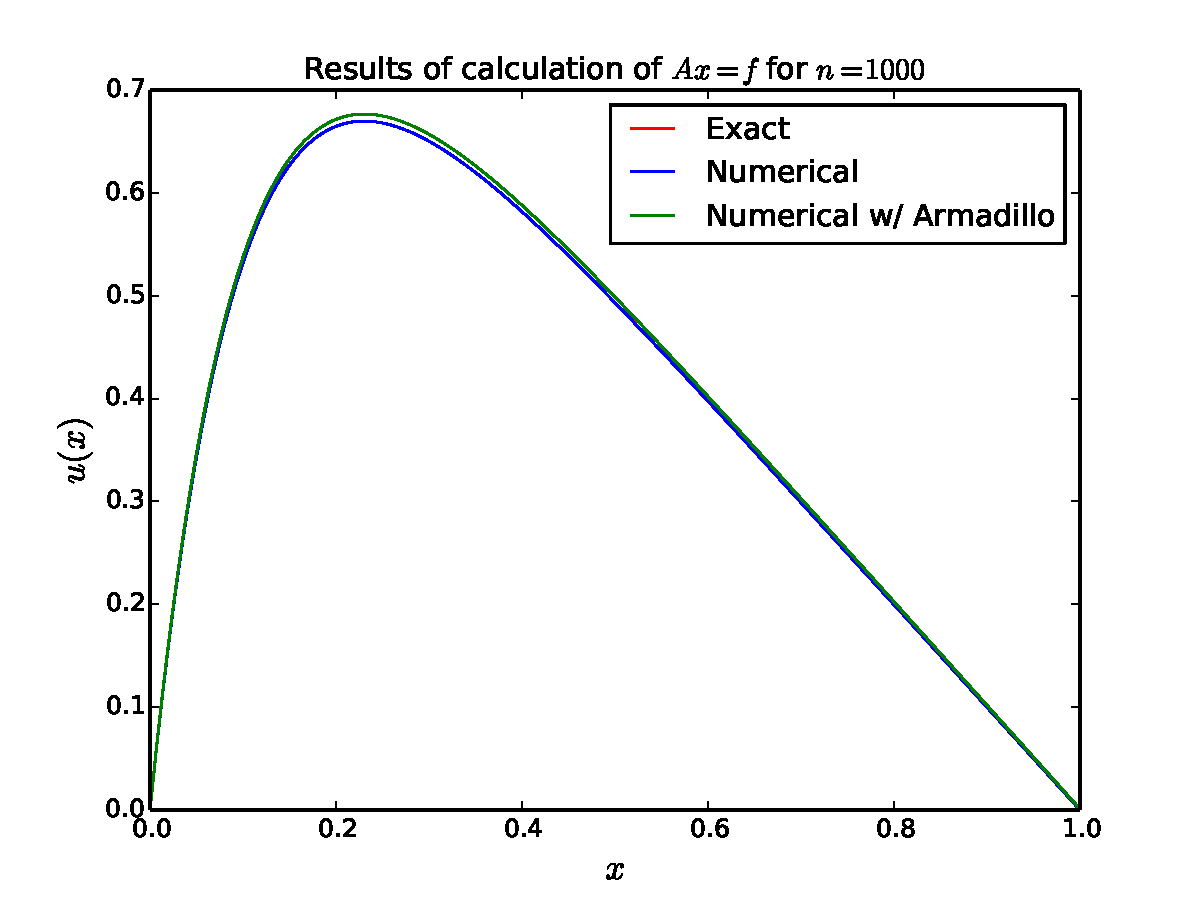
\includegraphics[width = .9\textwidth]{d_n_1000.pdf}
    \caption{Numerical solution for $n=10^3$.}
    \label{fig:sol103}
\end{figure}

\begin{figure}[H]
    \centering
    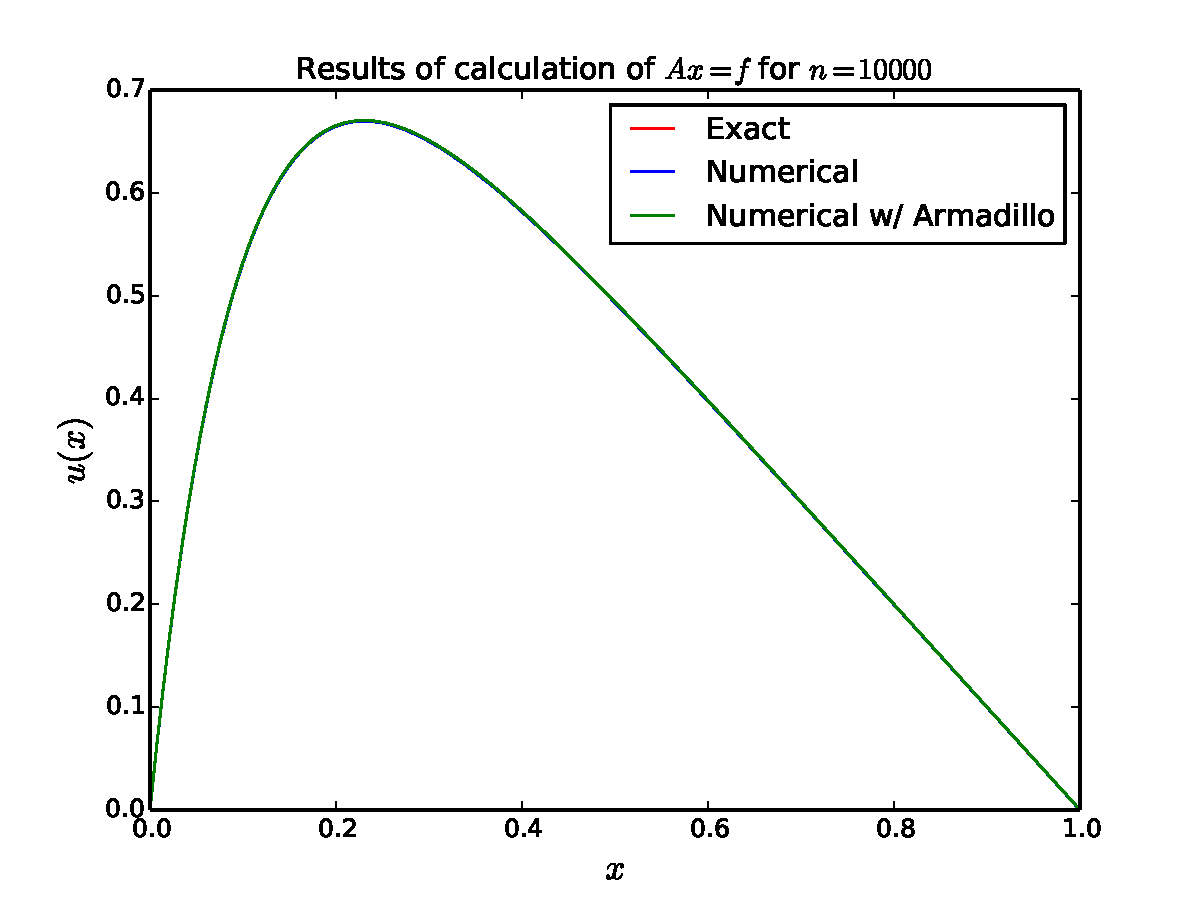
\includegraphics[width = .9\textwidth]{d_n_10000.pdf}
    \caption{Numerical solution for $n=10^4$.}
    \label{fig:sol104}
\end{figure}

Now we have seen that the precision of the two algorithms we've used are pretty different, now it's time to look at the time usage of the methods. Just for comparison I also added a function using LU-decomposition (see further down for code) for solving the equation. As mentioned earlier the LU-decomposition use $(2/3)n^3$ FLOPS while our own method use $8n$ FLOPS, it's pretty easy to guess which method is the fastest one.

In table \ref{tab:time} we see the results for different $n$. As expected the tridiagonal solver is the fastest one, and the LU-decomposition method is the slowest. When $n=10^4$ something strange happens to the time function in the library \verb|time.h|, it suddenly gives me a time far longer than it actually takes to run the program.

It could have been interesting to look how the time usage evolved with higher $n$, but the program crashes when I'm setting $n=10^5$. This may be due to memory handling and how I compile the program.

\begin{table}[H]
  \centering
  \begin{tabular}{ c c c c }
    \toprule
    $n$ & $t_{\text{Numerical}}$ & $t_{\text{Armadillo}}$ & $t_{\text{LU decomp.}}$ \\
    \midrule
	$10$   & $0.000002$ s & $0.000075$ s & $0.000123$ s \\
	$10^2$ & $0.000004$ s & $0.000701$ s & $0.002931$ s \\
	$10^3$ & $0.000027$ s & $0.068193$ s & $0.459989$ s \\
	$10^4$ & $0.000312$ s & $40.02037$ s & $297.6299$ s \\
    \bottomrule
  \end{tabular}
  \caption{Time spent by the different methods used to solve our problem. Something weird happens with the time-function when we set $n=10^4$ cause it didn't take five minutes to run the program on my own computer.}
  \label{tab:time}
\end{table}

Below the program for calculating the differential equation with LU-decomposition is listed. The program is using the LU-decomposition-functions from Armadillo. Mathematically it is done like this,

\begin{align*}
    Ax &= b \Rightarrow LUx = b \\
    Ux &= y  \Rightarrow Ly = b \\
    Ux &= L^{-1}b = y \Rightarrow x = U^{-1}y = U^{-1}L^{-1}b.
\end{align*}

\lstinputlisting[language=C++]{../lu_decomposition.cpp}

\section*{Conclusion} The far best method, of the two we tested properly in this project, for solving the differential equation $-u''(x) = f(x)$ is the tridiagonal solver. This gave us the most precise result -- if we should judge by looking at the plots -- and was also the fastest one. My project have some weaknesses, the algorithm could have been improved in order to reduce the number of FLOPS and the whole program could have been written with vectors instead of doubles, then it would have been easier to find index errors for example.
\newpage

\section{Python code for plotting}
\lstinputlisting[language=Python]{../plotting_results.py}
\end{document}